\documentclass[14pt]{beamer}
\usetheme{Dresden}
\usecolortheme{orchid}

\usepackage{xcolor}
\usepackage{listings}
\usepackage{courier}
\usepackage{graphicx}
\usepackage{amsmath}
\usepackage{algorithm2e}
\usepackage{multicol}

\usefonttheme[onlymath]{serif}

\definecolor{mGreen}{rgb}{0,0.6,0}
\definecolor{mGray}{rgb}{0.5,0.5,0.5}
\definecolor{mPurple}{rgb}{0.8,0,0.82}
\definecolor{backgroundColour}{rgb}{0.95,0.95,0.92}
\definecolor{lightBlue}{rgb}{0.1, 0.1, 0.8}

\lstdefinestyle{CStyle}{
    backgroundcolor=\color{backgroundColour},   
    commentstyle=\color{mGreen},
    keywordstyle=\color{magenta},
    numberstyle=\tiny\color{mGray},
    stringstyle=\color{mPurple},
    basicstyle=\footnotesize\ttfamily,
    breakatwhitespace=false,         
    breaklines=true,                 
    captionpos=b,                    
    keepspaces=true,                 
    numbers=left,                    
    numbersep=5pt,                  
    showspaces=false,                
    showstringspaces=false,
    showtabs=false,                  
    tabsize=2,
    language=C
}

\lstdefinestyle{Ctable}{
    backgroundcolor=\color{backgroundColour},   
    commentstyle=\color{mGreen},
    keywordstyle=\color{magenta},
    numberstyle=\tiny\color{mGray},
    stringstyle=\color{mPurple},
    basicstyle=\footnotesize\ttfamily,
    breakatwhitespace=false,         
    breaklines=true,                 
    captionpos=b,                    
    keepspaces=true,                                  
    showspaces=false,                
    showstringspaces=false,
    showtabs=false,                  
    tabsize=2,
    language=C
}

\lstdefinestyle{pseudo}{
        basicstyle=\ttfamily\footnotesize,
        keywordstyle=\color{lightBlue},
        morekeywords={BEGIN,END,IF,ELSE,ENDIF,ELSEIF,PRINT,WHILE,RETURN,ENDWHILE,DO,FOR,TO,IN,ENDFOR,BREAK,INPUT,READ},
        morecomment=[l]{//},
        commentstyle=\color{mGreen}
}

\lstset{basicstyle=\footnotesize\ttfamily,breaklines=true}
\lstset{framextopmargin=50pt,tabsize=2}

\title{ENGG1003 - Friday Week 3}
\subtitle{More Sequence Examples\\Maybe More Flow Control}
\author{Brenton Schulz}
\institute{University of Newcastle}
\date{\today}


\begin{document}
\titlepage


\begin{frame}
\frametitle{Assessment Task Rules}
\begin{center}
...Jump to rules PDF
\end{center}
\end{frame}

\begin{frame}
\frametitle{Easy(ish) Assessment Task Example}
{\small Write a C program which generates a sequence of numbers:
\begin{equation*}
x_1, x_2, x_3, ...
\end{equation*}
with the iterative equation:
\begin{equation*}
x_n = 3x_{n-1} + 2x_{n-2}
\end{equation*}
and initial conditions:
\begin{align*}
x_1 = 3,~ x_2 = 1
\end{align*}
The program should exit after printing ($x_8$ or an $x_n > 100$).
}
\end{frame}

\begin{frame}[fragile]
\frametitle{Easy(ish) Assessment Task Example}
The program's output format is:
\begin{lstlisting}[style=pseudo]
n x<newline>
\end{lstlisting}
For the values given, the output is:
\begin{lstlisting}[style=pseudo]
1 3.000000
2 1.000000
3 9.000000
4 29.000000
5 105.000000
\end{lstlisting}
\end{frame}

\begin{frame}
\frametitle{Easy(ish) Assessment Task Example}
\begin{itemize}
\item What do we need to do?
	\begin{itemize}
		\item Set up variables
		\item Give some initial values
		\item Implement the equation
		\item Print the initial values
		\item Write a \texttt{while()} loop
		\item Get the exit condition correct
		\item Print results
		\item Wrap the whole thing in \texttt{main()}
	\end{itemize}
\end{itemize}
\end{frame}

\begin{frame}[fragile]
\frametitle{Set up variables}
Question didn't specify, but lets assume \texttt{float}
\begin{lstlisting}[style=CStyle]
float xn, xnm1, xnm2;
int n; 
\end{lstlisting}
\end{frame}

\begin{frame}[fragile]
\frametitle{Give some initial values}
Question gave us:
\begin{align*}
x_1 = 3,~ x_2 = 1
\end{align*}
Be careful with \texttt{xnm1} and \texttt{xnm2}, where are we starting? 
\begin{lstlisting}[style=CStyle]
float xn, xnm1 = 1, xnm2 = 3;
int n = 3; // The first unknown is x for n=3
\end{lstlisting}
\end{frame}

\begin{frame}[fragile]
\frametitle{Implement the equation}
\begin{equation*}
x_n = 3x_{n-1} + 2x_{n-2}
\end{equation*}
\begin{lstlisting}[style=CStyle]
float xn, xnm1 = 1, xnm2 = 3;
int n = 3; // The first unknown is x for n=3

xn = 3.0*xnm1 + 2*xnm2;
\end{lstlisting}
That calculates $x_3$, but how does the program ``advance in time''?
\end{frame}

\begin{frame}[fragile]
\frametitle{Implement the equation}
Shift all the variables ``forward in time'' with:
\begin{lstlisting}[style=CStyle]
float xn, xnm1 = 1, xnm2 = 3;
int n = 3; // The first unknown is x for n=3

xn = 3.0*xnm1 + 2*xnm2;
xnm2 = xnm1;
xnm1 = xn;
\end{lstlisting}
\end{frame}

\begin{frame}[fragile]
\frametitle{Print the initial values}
\begin{lstlisting}[style=CStyle]
float xn, xnm1 = 1, xnm2 = 3;
int n = 3; // The first unknown is x for n=3

// x1 and x2 given so just hard code n
printf("1 %f\n", xnm2);
printf("2 %f\n", xnm1);

xn = 3.0*xnm1 + 2*xnm2;
xnm2 = xnm1;
xnm1 = xn;
\end{lstlisting}
\end{frame}

\begin{frame}[fragile]
\frametitle{Write a \texttt{while()} loop}
We need to calculate $x_n$ more than once, so:
\begin{lstlisting}[style=CStyle]
float xn, xnm1 = 1, xnm2 = 3;
int n = 3; // The first unknown is x for n=3

// x1 and x2 given so just hard code n
printf("1 %f\n", xnm2);
printf("2 %f\n", xnm1);

while( /* something */ ) {
	xn = 3.0*xnm1 + 2*xnm2;
	xnm2 = xnm1;
	xnm1 = xn;
}
\end{lstlisting}
\end{frame}

\begin{frame}[fragile]
\frametitle{Get the exit condition correct}
The value of n goes from 1 to 8, and xn must remain below 100:
\begin{lstlisting}[style=CStyle]
float xn, xnm1 = 1, xnm2 = 3;
int n = 3; // The first unknown is x for n=3
// x1 and x2 given so just hard code n
printf("1 %f\n", xnm2);
printf("2 %f\n", xnm1);
while( (n <= 8) && (xn < 100) ) {
	xn = 3.0*xnm1 + 2*xnm2;
	xnm2 = xnm1;
	xnm1 = xn;
	n++;
}
\end{lstlisting}
\end{frame}

\begin{frame}[fragile]
\frametitle{Print results}
\begin{lstlisting}[style=CStyle]
float xn, xnm1 = 1, xnm2 = 3;
int n = 3; // The first unknown is x for n=3
// x1 and x2 given so just hard code n
printf("1 %f\n", xnm2);
printf("2 %f\n", xnm1);
while( (n <= 8) && (xn < 100) ) {
	xn = 3.0*xnm1 + 2*xnm2;
	xnm2 = xnm1;
	xnm1 = xn;
	n++;
	printf("%d %f\n", n, xn);
}
\end{lstlisting}
\end{frame}

\begin{frame}[fragile]
\frametitle{Wrap the whole thing in \texttt{main()}}
\textbf{NB:} This code still has errors. Debugged version in Che, see recording.
{\small
\begin{lstlisting}[style=CStyle]
#include <stdio.h>
main() {
	float xn, xnm1 = 1, xnm2 = 3;
	int n = 3; // The first unknown is x for n=3
	// x1 and x2 given so just hard code n
	printf("1 %f\n", xnm2);
	printf("2 %f\n", xnm1);
	while( (n <= 8) && (xn < 100) ) {
		xn = 3.0*xnm1 + 2*xnm2;
		xnm2 = xnm1;
		xnm1 = xn;
		n++;
		printf("%d %f\n", n, xn);
	}
}
\end{lstlisting}
}
\end{frame}

\begin{frame}[fragile]
\frametitle{Is the solution optimal?}
\begin{itemize}
\item Some marks are allocated to reducing variable count
\item It tests your understanding of how the \texttt{=} operation works
\item Lets look at the maths:
\begin{lstlisting}[style=CStyle]
xn = 3.0*xnm1 + 2*xnm2;
xnm2 = xnm1;
xnm1 = xn;
n++;
printf("%d %f\n", n, xn);
\end{lstlisting}
\item Do we need \textit{all} those variables?
\end{itemize}
\end{frame}

\begin{frame}[fragile]
\begin{itemize}
\item In this case: yes
\begin{lstlisting}[style=CStyle]
xn = 3.0*xnm1 + 2*xnm2;
xnm2 = xnm1;
xnm1 = xn;
n++;
printf("%d %f\n", n, xn);
\end{lstlisting}
\item We can't overwrite \texttt{xnm1} before shifting it into \texttt{xnm2}
\item Result must be stored in \texttt{xn} first
\end{itemize}
\end{frame}

\begin{frame}[fragile]
\frametitle{Another Isolated Example}
\begin{itemize}
\item What if the equation was:
\begin{equation*}
x_n = 0.2x_{n-1}
\end{equation*}
\item This will \textit{work}:

\begin{lstlisting}[style=CStyle]
xn = 0.2*xnm1;
xnm1 = xn;
\end{lstlisting}

\item But because we never need \texttt{xnm1} elsewhere this is more optimal:
\begin{lstlisting}[style=CStyle]
xn = 0.2*xn;
\end{lstlisting}
\item Marks (above a pass) may be allocated to variable optimisation
\end{itemize}
\end{frame}

\begin{frame}[fragile]
\frametitle{Hard Assessment Task Example}
{\small Write a C program which generates two sequences of numbers:
\begin{align*}
& x_0, x_1, x_2, ...\\
& y_0, y_1, y_2, ...
\end{align*}
with the coupled iterative equations:
\begin{align*}
x_n &= 0.6x_{n-1} + 0.2y_{n-1}\\
y_n &= 0.1x_{n-1} + 0.9y_{n-1}
\end{align*}
and initial conditions:
\begin{align*}
x_0 &= 5\\
y_0 &= 0
\end{align*}
}
\end{frame}

\begin{frame}
\frametitle{Hard Assessment Task Example}
\begin{align*}
x_n &= 0.6x_{n-1} + 0.2y_{n-1}\\
y_n &= 0.1x_{n-1} + 0.9y_{n-1}
\end{align*}
\vspace{-6mm}
\begin{itemize}
\item Lets have an attempt at implementing the equations
\item We need \textit{at least} two variables:
	\begin{itemize}
		\item \texttt{float xn}
		\item \texttt{float yn}
	\end{itemize}
\item Lets also use two ``previous'' variables:
	\begin{itemize}
		\item \texttt{float xnm1}
		\item \texttt{float ynm1}
	\end{itemize}	
\end{itemize}
\end{frame}

\begin{frame}[fragile]
\frametitle{Hard Assessment Task Example}
\begin{align*}
x_n &= 0.6x_{n-1} + 0.2y_{n-1}\\
y_n &= 0.1x_{n-1} + 0.9y_{n-1}
\end{align*}
\vspace{-6mm}
\begin{itemize}
\item Our calculation code can then be:
\begin{lstlisting}[style=CStyle]
xn = 0.6*xnm1 + 0.2*ynm1;
yn = 0.1*xnm1 + 0.9*ynm1;
xnm1 = xn;
ynm1 = yn;
\end{lstlisting}
\item \textbf{Question:} Do we need all these variables?
\end{itemize}
\end{frame}

\begin{frame}[fragile]
\frametitle{Hard Assessment Task Example}
\vspace{-5mm}
\begin{align*}
x_n &= 0.6x_{n-1} + 0.2y_{n-1}\\
y_n &= 0.1x_{n-1} + 0.9y_{n-1}
\end{align*}
\vspace{-6mm}
\begin{itemize}
\item \textbf{Counter-question:} What is wrong with this?
\begin{lstlisting}[style=CStyle]
xn = 0.6*xn + 0.2*yn;
yn = 0.1*xn + 0.9*yn;
\end{lstlisting}
\pause
\item Why doesn't mathematics convert into code?
\end{itemize}
\end{frame}

\begin{frame}[fragile]
\frametitle{Hard Assessment Task Example}
\begin{itemize}
\item Mathematics is \textit{instant}
\pause
\item Code is evaluated line by line
\pause
\item Variables can \textit{change} between lines, resulting in the wrong equation being implemented
\item The previous slide was \textit{actually} doing:
\end{itemize}

\begin{multicols}{2}
\begin{align*}
x_n &= 0.6x_{n-1} + 0.2y_{n-1}\\
y_n &= 0.1\textcolor{red}{x_{n}} + 0.9y_{n-1}
\end{align*}
~\\~\\
\begin{lstlisting}[style=pseudo]
xn = 0.6*xn + 0.2*yn;
yn = 0.1*xn + 0.9*yn;
\end{lstlisting}
\end{multicols}


\end{frame}

\begin{frame}
\frametitle{Hard Assessment Task Example}
\begin{itemize}
\item Observe the correct subscripts:
\begin{align*}
x_n &= 0.6x_{n-1} + 0.2y_{n-1}\\
y_n &= 0.1\textcolor{red}{x_{n-1}} + 0.9y_{n-1}
\end{align*}
\item In the 2nd equation we need $x_{n-1}$ but the first equation would destroy that value
\item We \textit{must} use an extra variable to store $x_{n-1}$ for $y_n$ to be calculated correctly
\end{itemize}
\end{frame}

\begin{frame}[fragile]
\frametitle{Hard Assessment Task Example}
\begin{itemize}
\item Aside: You may see coupled equations vaguely like this in signals and systems theory
\begin{align*}
x_n &= 0.6x_{n-1} + 0.2y_{n-1}\\
y_n &= 0.1x_{n-1} + 0.9y_{n-1}
\end{align*}

\item Lets write C code with the minimum variables:
\begin{lstlisting}[style=pseudo]
xtmp = x;	// store xn before we lose it
x = 0.6*x + 0.2*y;	// Original xn value lost
y = 0.1*xtmp + 0.9*y;	// stored xn used, yn
\end{lstlisting}
\item ...And implement in Che
\end{itemize}
\end{frame}

\begin{frame}
\frametitle{Results}
\begin{center}
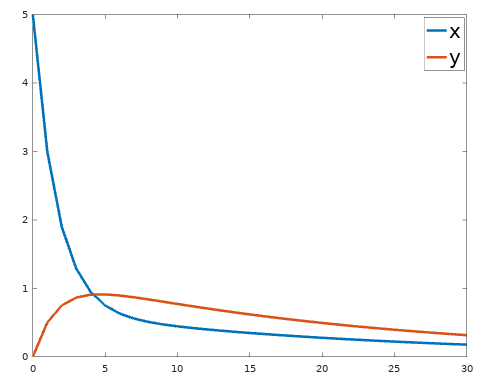
\includegraphics[width=0.6\textwidth]{coupled}\\
{\small Aside: results data was pulled from Che using SSH. Advanced students will appreciate this feature in later weeks.}
\end{center}
\end{frame}

\end{document}
